\documentclass[12pt,dvipdfmx]{beamer}
\institute{}
\author{田浦健次朗}
\date{}

\usepackage{graphicx}
\DeclareGraphicsExtensions{.pdf}
\DeclareGraphicsExtensions{.eps}
\graphicspath{{out/}{out/tex/}{out/tex/gpl/}{out/tex/svg/}{out/tex/lsvg/}{out/tex/dot/}}
% \graphicspath{{out/}{out/tex/}{out/pdf/}{out/eps/}{out/tex/gpl/}{out/tex/svg/}{out/pdf/dot/}{out/pdf/gpl/}{out/pdf/img/}{out/pdf/odg/}{out/pdf/svg/}{out/eps/dot/}{out/eps/gpl/}{out/eps/img/}{out/eps/odg/}{out/eps/svg/}}
\usepackage{listings,jlisting}
\usepackage{fancybox}
\usepackage{hyperref}
\usepackage{color}

%%%%%%%%%%%%%%%%%%%%%%%%%%%
%%% themes
%%%%%%%%%%%%%%%%%%%%%%%%%%%
\usetheme{default} % Szeged
%% no navigation bar
% default boxes Bergen Boadilla Madrid Pittsburgh Rochester
%% tree-like navigation bar
% Antibes JuanLesPins Montpellier
%% toc sidebar
% Berkeley PaloAlto Goettingen Marburg Hannover Berlin Ilmenau Dresden Darmstadt Frankfurt Singapore Szeged
%% Section and Subsection Tables
% Copenhagen Luebeck Malmoe Warsaw

%%%%%%%%%%%%%%%%%%%%%%%%%%%
%%% innerthemes
%%%%%%%%%%%%%%%%%%%%%%%%%%%
% \useinnertheme{circles}	% default circles rectangles rounded inmargin

%%%%%%%%%%%%%%%%%%%%%%%%%%%
%%% outerthemes
%%%%%%%%%%%%%%%%%%%%%%%%%%%
% outertheme
% \useoutertheme{default}	% default infolines miniframes smoothbars sidebar sprit shadow tree smoothtree


%%%%%%%%%%%%%%%%%%%%%%%%%%%
%%% colorthemes
%%%%%%%%%%%%%%%%%%%%%%%%%%%
\usecolortheme{seahorse}
%% special purpose
% default structure sidebartab 
%% complete 
% albatross beetle crane dove fly seagull 
%% inner
% lily orchid rose
%% outer
% whale seahorse dolphin

%%%%%%%%%%%%%%%%%%%%%%%%%%%
%%% fontthemes
%%%%%%%%%%%%%%%%%%%%%%%%%%%
\usefonttheme{serif}  
% default professionalfonts serif structurebold structureitalicserif structuresmallcapsserif

%%%%%%%%%%%%%%%%%%%%%%%%%%%
%%% generally useful beamer settings
%%%%%%%%%%%%%%%%%%%%%%%%%%%
% 
\AtBeginDvi{\special{pdf:tounicode EUC-UCS2}}
% do not show navigation
\setbeamertemplate{navigation symbols}{}
% show page numbers
\setbeamertemplate{footline}[frame number]

%%%%%%%%%%%%%%%%%%%%%%%%%%%
%%% define some colors for convenience
%%%%%%%%%%%%%%%%%%%%%%%%%%%

\newcommand{\mido}[1]{{\color{green}#1}}
\newcommand{\mura}[1]{{\color{purple}#1}}
\newcommand{\ore}[1]{{\color{orange}#1}}
\newcommand{\ao}[1]{{\color{blue}#1}}
\newcommand{\aka}[1]{{\color{red}#1}}

\setbeamercolor{ex}{bg=cyan!20!white}

\definecolor{UniBlue}{RGB}{20,20,250} 
\setbeamercolor{structure}{fg=UniBlue} % 見出しカラー

\iffalse
%%%%%%%%%%%%%%%%%%%%%%%%%%%
%% customize beamer template
%% https://www.opt.mist.i.u-tokyo.ac.jp/~tasuku/beamer.html
%%%%%%%%%%%%%%%%%%%%%%%%%%%

%\renewcommand{\familydefault}{\sfdefault}  % 英文をサンセリフ体に
%\renewcommand{\kanjifamilydefault}{\gtdefault}  % 日本語をゴシック体に
\usefonttheme{structurebold} % タイトル部を太字
\setbeamerfont{alerted text}{series=\bfseries} % Alertを太字
\setbeamerfont{section in toc}{series=\mdseries} % 目次は太字にしない
\setbeamerfont{frametitle}{size=\Large} % フレームタイトル文字サイズ
\setbeamerfont{title}{size=\LARGE} % タイトル文字サイズ
\setbeamerfont{date}{size=\small}  % 日付文字サイズ

\definecolor{UniBlue}{RGB}{0,150,200} 
\definecolor{AlertOrange}{RGB}{255,76,0}
\definecolor{AlmostBlack}{RGB}{38,38,38}
\setbeamercolor{normal text}{fg=AlmostBlack}  % 本文カラー
\setbeamercolor{structure}{fg=UniBlue} % 見出しカラー
\setbeamercolor{block title}{fg=UniBlue!50!black} % ブロック部分タイトルカラー
\setbeamercolor{alerted text}{fg=AlertOrange} % \alert 文字カラー
\mode<beamer>{
    \definecolor{BackGroundGray}{RGB}{254,254,254}
    \setbeamercolor{background canvas}{bg=BackGroundGray} % スライドモードのみ背景をわずかにグレーにする
}


%フラットデザイン化
\setbeamertemplate{blocks}[rounded] % Blockの影を消す
\useinnertheme{circles} % 箇条書きをシンプルに
\setbeamertemplate{navigation symbols}{} % ナビゲーションシンボルを消す
\setbeamertemplate{footline}[frame number] % フッターはスライド番号のみ

%タイトルページ
\setbeamertemplate{title page}{%
    \vspace{2.5em}
    {\usebeamerfont{title} \usebeamercolor[fg]{title} \inserttitle \par}
    {\usebeamerfont{subtitle}\usebeamercolor[fg]{subtitle}\insertsubtitle \par}
    \vspace{1.5em}
    \begin{flushright}
        \usebeamerfont{author}\insertauthor\par
        \usebeamerfont{institute}\insertinstitute \par
        \vspace{3em}
        \usebeamerfont{date}\insertdate\par
        \usebeamercolor[fg]{titlegraphic}\inserttitlegraphic
    \end{flushright}
}
\fi

%%%%%%%%%%%%%%%%%%%%%%%%%%%
%%% how to typset code
%%%%%%%%%%%%%%%%%%%%%%%%%%%

\lstset{language = C,
numbers = left,
numberstyle = {\tiny \emph},
numbersep = 10pt,
breaklines = true,
breakindent = 40pt,
frame = tlRB,
frameround = ffft,
framesep = 3pt,
rulesep = 1pt,
rulecolor = {\color{blue}},
rulesepcolor = {\color{blue}},
flexiblecolumns = true,
keepspaces = true,
basicstyle = \ttfamily\scriptsize,
identifierstyle = ,
commentstyle = ,
stringstyle = ,
showstringspaces = false,
tabsize = 4,
escapechar=\@,
}

\AtBeginSection[]
{
\begin{frame}
\frametitle{}
\tableofcontents[currentsection]
\end{frame}
}

\AtBeginSubsection[]
{
\begin{frame}
\frametitle{}
\tableofcontents[currentsection,currentsubsection]
\end{frame}
}


\title{ファイルシステム}
\begin{document}
\maketitle

%%%%%%%%%%%%%%%%%%%%%%%%%%%%%%%%%% 
\begin{frame}
\frametitle{目次}
\tableofcontents
\end{frame}

%%%%%%%%%%%%%%%%% 
\section{ファイルシステムの役割}
%%%%%%%%%%%%%%%%% 

%%%%%%%%%%%%%%%%% 
\begin{frame}
  \frametitle{ファイルシステムとは}
  \begin{columns}
    \begin{column}{0.5\textwidth}
      \begin{itemize}
      \item 第一義的には, 2次記憶装置に対してOSが提供している抽象化
      \item 2次記憶装置
        \begin{itemize}
        \item ハードディスク
        \item SSD
        \item USBメモリ
        \item SD card
        \item etc.
        \end{itemize}
      \item 色々な2次記憶装置を\ao{簡便}な,
        \ao{共通}のインタフェースで読めるようにする
      \end{itemize}
    \end{column}
    \begin{column}{0.5\textwidth}
      \includegraphics[width=\textwidth]{out/pdf/svg/file_system_1.pdf}
    \end{column}
  \end{columns}
\end{frame}

%%%%%%%%%%%%%%%%% 
\begin{frame}
  \frametitle{ファイルシステムが提供する基本的な抽象化}
  \begin{itemize}
  \item \ao{ファイル}
    \begin{itemize}
    \item $\approx$ 自由に伸縮できるバイト配列
    \end{itemize}
  \item \ao{ディレクトリ, フォルダ} (階層構造)
    \begin{itemize}
    \item 他のファイルやディレクトリを含むことが出来る「入れ物」
    \end{itemize}
  \item 名前空間
    \begin{itemize}
    \item ファイル, ディレクトリに名前を付けられる
    \end{itemize}
  \end{itemize}
  \begin{center}
    \includegraphics[width=0.45\textwidth]{out/pdf/svg/file_system_2.pdf}
  \end{center}
\end{frame}

%%%%%%%%%%%%%%%%% 
\section{ファイルシステムのAPI}
%%%%%%%%%%%%%%%%% 

%%%%%%%%%%%%%%%%% 
\begin{frame}
  \frametitle{open, close}
  \begin{itemize}
  \item \ao{\tt int {\it fd} = open({\it path}, {\it flags}{\rm [, {\it mode}]});}
    \begin{itemize}
    \item {\it path}で指定されるファイルを開く, 場合により, 新たに作る
    \item 成功すれば, 後に{\tt read/write}などに渡せる,
      \ao{ファイルディスクリプタ}{\it fd}を返す (実体はただの整数)
    \item {\it flags}
      \begin{itemize}
      \item {\tt O\_RDONLY, O\_WRONLY, O\_RDWR} : 読むだけ, 書くだけ, 両方
      \item {\tt O\_CREAT} : 存在しなければ作る
      \item {\tt O\_EXCL} : 存在していたらエラー
      \item {\tt O\_TRUNC} : 存在していたら一旦空(0バイト)にする
      \item etc.
      \end{itemize}
    \end{itemize}
  \item ファイルディスクリプタ(openされたファイル)に紐付いている情報
    \begin{itemize}
    \item \ao{ファイルオフセット} : 次の読み書きが行われる場所
    \item open直後は0
    \end{itemize}
  \end{itemize}
\end{frame}

%%%%%%%%%%%%%%%%% 
\begin{frame}
  \frametitle{ファイルシステムの構成とパス(path)について}
  \begin{itemize}
  \item ファイルシステム全体は, 一つの大きな木構造
  \item 木構造の
    \begin{itemize}
    \item リーフが(通常の)\ao{ファイル}
    \item リーフでない内部ノードは, \ao{ディレクトリ(フォルダとも言う)}
    \end{itemize}
  \end{itemize}
  \begin{columns}
    \begin{column}{0.65\textwidth}
      \begin{itemize}
      \item 任意のファイル・ディレクトリは木構造の根(\ao{ルートディレクトリ}という)
        からそれに至る道(\ao{絶対パス})を指定することで一意に特定可能
        \begin{itemize}
        \item 絶対パスの例 {\tt /usr/bin/python} : ルートディレクトリ内の{\tt usr}内の{\tt bin}内の{\tt python}
        \end{itemize}
      \end{itemize}      
    \end{column}
    \begin{column}{0.35\textwidth}
      \begin{center}
        \includegraphics[width=\textwidth]{out/pdf/svg/file_system_3.pdf}
      \end{center}
    \end{column}
  \end{columns}
\end{frame}

%%%%%%%%%%%%%%%%% 
\begin{frame}
  \frametitle{相対パスとカレントディレクトリ}
  \begin{itemize}
  \item 任意のディレクトリを起点としたファイル・ディレクトリへのパスを
    \ao{相対パス}という
  \item 特に親ディレクトリを {\tt ..} というパスで指定する
  \item これで, 任意の起点から任意のファイル・ディレクトリを指定可能
  \end{itemize}
  \begin{columns}
    \begin{column}{0.60\textwidth}
      \begin{itemize}
      \item 各プロセスは「現在のディレクトリ」(\ao{カレントディレクトリ})
        という属性があり, 相対パスは, 通常カレントディレクトリからの相対パス
      \item カレントディレクトリの変更: {\tt chdir} システムコール,
        シェルの {\tt cd} コマンド
      \end{itemize}
    \end{column}
    \begin{column}{0.40\textwidth}
      \begin{center}
        \includegraphics[width=\textwidth]{out/pdf/svg/file_system_4.pdf}
      \end{center}
    \end{column}
  \end{columns}
\end{frame}

%%%%%%%%%%%%%%%%% 
\begin{frame}
  \frametitle{read, write}
  \begin{itemize}
  \item<1-> \ao{\tt ssize\_t {\it r} = read({\it fd}, {\it buf}, {\it sz});}
    \begin{itemize}
    \item ファイルオフセットから最大{\it sz}バイト, 
      {\it buf}から始まる領域に読み込む
    \item 実際に読み込まれたバイト数を返す
    \item ファイルオフセットが{\it r}前進
    \end{itemize}
  \item<3-> \ao{\tt ssize\_t {\it w} = write({\it fd}, {\it buf}, {\it sz});}
    \begin{itemize}
    \item {\it buf}から始まる領域から, 最大{\it sz}バイトを,
      ファイルオフセットに書き込む
    \item 場合によりファイルが伸長する
    \item 実際に書き込まれたバイト数を返す
    \item ファイルオフセットが{\it w}前進
    \end{itemize}
  \end{itemize}
  \begin{center}
    \only<1>{\includegraphics[width=0.6\textwidth]{out/pdf/svg/read_write_1.pdf}}%
    \only<2>{\includegraphics[width=0.6\textwidth]{out/pdf/svg/read_write_2.pdf}}%
    \only<3>{\includegraphics[width=0.6\textwidth]{out/pdf/svg/read_write_3.pdf}}%
    \only<4>{\includegraphics[width=0.6\textwidth]{out/pdf/svg/read_write_4.pdf}}%
    \only<5>{\includegraphics[width=0.6\textwidth]{out/pdf/svg/read_write_5.pdf}}%
    \only<6->{\includegraphics[width=0.6\textwidth]{out/pdf/svg/read_write_6.pdf}}%
  \end{center}
\end{frame}

%%%%%%%%%%%%%%%%% 
\begin{frame}
  \frametitle{lseek}
  \begin{itemize}
  \item \ao{\tt off\_t {\it o} = lseek({\it fd}, {\it offset}, {\it whence});}
    \begin{itemize}
    \item ファイルオフセット(次にread/writeが作用する場所)を
      {\it whence}に応じた{\it offset}にする
    \item これで, ファイルの一部だけを読み書きできる
    \item {\tt SEEK\_SET} : ファイル先頭から
    \item {\tt SEE\_CUR} : 現在位置から
    \item {\tt SEEK\_END} : ファイルの終わりから
    \end{itemize}
  \end{itemize}
  \begin{center}
    \only<1>{\includegraphics[width=0.6\textwidth]{out/pdf/svg/read_write_7.pdf}}%
    \only<2->{\includegraphics[width=0.6\textwidth]{out/pdf/svg/read_write_8.pdf}}%
  \end{center}
\end{frame}

%%%%%%%%%%%%%%%%% 
\begin{frame}
  \frametitle{read, writeの変種 --- pread, pwrite}
  \begin{itemize}
  \item {\tt ssize\_t {\it r} = pread({\it fd}, {\it buf}, {\it sz}, \ao{\it offset});}
    \begin{itemize}
    \item \ao{\it offset}から最大{\it sz}バイト, 
      {\it buf}から始まる領域に読み込む
    \item 実際に読み込まれたバイト数を返す
    \item ファイルオフセットは\ao{変わらない}
    \end{itemize}
  \item {\tt ssize\_t {\it w} = pwrite({\it fd}, {\it buf}, {\it sz}, \ao{\it offset});}
    \begin{itemize}
    \item {\it buf}から始まる領域から, 最大{\it sz}バイトを,
      \ao{\it offset}に書き込む
    \item 場合によりファイルが伸長する
    \item 実際に書き込まれたバイト数を返す
    \item ファイルオフセットは\ao{変わらない}
    \end{itemize}
  \item 存在理由
    \begin{itemize}
    \item 逐次的でない読み書きをするときは lseek + read/write よりも簡潔
    \item (重要) 複数のスレッドが同じ {\it fd} から読み書きするとき
      (lssek/read/writeで,
      ファイルオフセットが変化するというインタフェースが扱いづらい)
    \end{itemize}
  \end{itemize}
\end{frame}

%%%%%%%%%%%%%%%%% 
\begin{frame}
  \frametitle{read, writeの変種 --- readv, writev}
  \begin{itemize}
  \item 複数のread, writeを一撃で実行できる
    (複数の {\it buf, sz} ({\tt iovec} 構造体) を与えることができる)
  \item 詳細はman pageを参照
  \item preadv, pwritev もある
  \end{itemize}
\end{frame}


%%%%%%%%%%%%%%%%% 
\begin{frame}
  \frametitle{fallocate, ftruncate}
  \begin{itemize}
  \item \ao{\tt int $e$ = posix\_fallocate({\it fd}, {\it offset}, {\it len});}
  \item \ao{\tt int $e$ = fallocate({\it fd}, {\it mode}, {\it offset}, {\it len});}
    \begin{itemize}
    \item ファイルの$[{\it offset}, {\it offset+len})$バイトの範囲を,
      必要ならばファイルを伸長し, 0にする
    \item {\tt fallocate}はLinux固有 (man -s 2 ftruncate参照)
    \end{itemize}
    
  \item<3-> \ao{\tt int $e$ = ftruncate({\it fd}, off\_t {\it len});}
    \begin{itemize}
    \item ファイルの大きさを{\it len}バイトに,
      短縮(伸長できるOSもある)する
    \end{itemize}
  \end{itemize}
  \begin{center}
    \only<1>{\includegraphics[width=0.6\textwidth]{out/pdf/svg/read_write_9.pdf}}%
    \only<2>{\includegraphics[width=0.6\textwidth]{out/pdf/svg/read_write_10.pdf}}%
    \only<3>{\includegraphics[width=0.6\textwidth]{out/pdf/svg/read_write_11.pdf}}%
    \only<4->{\includegraphics[width=0.6\textwidth]{out/pdf/svg/read_write_12.pdf}}%
  \end{center}
\end{frame}

%%%%%%%%%%%%%%%%% 
\begin{frame}
  \frametitle{close, unlink}
  \begin{itemize}
  \item \ao{\tt int {\it e} = close({\it fd});}
    \begin{itemize}
    \item openしたファイルを閉じる({\it fd}が無効になり,
      以降のopenにおける再利用の対象になる)
    \end{itemize}
  \item \ao{\tt int {\it e} = unlink({\it path});}
    \begin{itemize}
    \item $\approx$ ファイルを消す
    \end{itemize}
  \end{itemize}
\end{frame}

%%%%%%%%%%%%%%%%% 
\begin{frame}
  \frametitle{mmap}
  \begin{itemize}
  \item 有用かつ奥深いAPI
  \item 色々な役割を兼ねる
    \begin{enumerate}
    \item ファイルを「メモリ上にあるかのように」読み書きする
    \item メモリを割り当てる(sbrkの役割を兼ねる)
    \item 割り当てるアドレスを指定する(疎なアドレス空間)
    \item 読み書き保護を設定する
    \end{enumerate}
  \end{itemize}
\end{frame}

%%%%%%%%%%%%%%%%% 
\begin{frame}
  \frametitle{mmap API 基本}
  \begin{itemize}
  \item \ao{\tt void * {\it a} = mmap($a_0$, {\it len}, {\it prot}, {\it flags}, {\it fd}, {\it o});}
  \item \ao{基本:} {\it fd}に対応するファイルの{\it o}
    バイト目から{\it len}バイトが,
    返り値のアドレス$a$に\ao{「対応付けられる(マップされる)」}
  \item $\iff$  $a[i]$がファイルの({\it o $+$ i})バイト目に対応
  \item 返り値 ($a$) これまで使われていなかったアドレス
  \item すなわち, \ao{メモリが新たに割り当てられる}効果も持つ
  \end{itemize}
  \begin{center}
    \only<1>{\includegraphics[width=0.8\textwidth]{out/pdf/svg/mmap_1.pdf}}%
    \only<2->{\includegraphics[width=0.8\textwidth]{out/pdf/svg/mmap_2.pdf}}
  \end{center}
\end{frame}

%%%%%%%%%%%%%%%%% 
\begin{frame}
  \frametitle{mmap API オプション}
  \begin{itemize}
  \item \ao{\tt void * {\it a} = mmap($a_0$, {\it len}, {\it prot}, {\it flags}, {\it fd}, {\it o});}
  \item \ao{\it prot} : 割り当てられた領域の保護属性
    \begin{itemize}
    \item {\tt PROT\_EXEC} : (命令として)実行可能にする
    \item {\tt PROT\_READ} : 読み出し可能にする
    \item {\tt PROT\_WRITE} : 書き込み可能にする
    \end{itemize}
    
  \item \ao{\it flags} : {\tt MAP\_SHARED} または {\tt MAP\_PRIVATE}を指定;
    複数プロセスが同じ領域をmmapした場合,
    \begin{itemize}
    \item {\tt MAP\_SHARED}
      $a[i]$への書き込みは, 
      \begin{enumerate}
      \item ファイルへ反映される
      \item それらのプロセス間で共有される
      \end{enumerate}
    \item {\tt MAP\_PRIVATE}
      $a[i]$への書き込みは, 
      \begin{enumerate}
      \item ファイルへ反映されない
      \item それらのプロセス間でも共有されない
      \end{enumerate}
    \item その他のフラグは後述
    \end{itemize}
  \end{itemize}
\end{frame}

%%%%%%%%%%%%%%%%% 
\begin{frame}
  \frametitle{mmap API アドレスの指定}
  \begin{itemize}
  \item \ao{$a_0$}
    \begin{itemize}
    \item $a_0 (\neq 0)$ $\rightarrow$
      アドレス$a_0$を割り当てるよう指定($a_0$が空いていない場合はエラー)
    \item $a_0 = 0$ $\rightarrow$
      OSが, 空いているところを割り当てる
    \end{itemize}
  \end{itemize}
  \begin{center}
    \includegraphics[width=0.8\textwidth]{out/pdf/svg/mmap_3.pdf}
  \end{center}
\end{frame}

%%%%%%%%%%%%%%%%% 
\begin{frame}[fragile]
  \frametitle{mmapでファイル読み出し}
  \begin{itemize}
  \item []
\begin{lstlisting}
int fd = open(@{\it filename}@, O_RDONLY);
struct stat sb[1];
@\ao{\tt fstat}@(fd, sb);
long sz = sb->st_size;
char * a = mmap(0, sz, PROT_READ, MAP_PRIVATE, fd, 0);
/* filenameのiバイト目がa[i]で読み出せる */
for (long i = 0; i < sz; i++) {
  putchar(a[i]);
}
\end{lstlisting}
\item 注: エラーチェックは省略(以下同様)
\item エラーチェックのやり方({\tt man err}参照)
\begin{lstlisting}
if (fstat(fd, sb) == -1) err(1, "fstat");
\end{lstlisting}
\end{itemize}
\end{frame}

%%%%%%%%%%%%%%%%% 
\begin{frame}[fragile]
  \frametitle{mmapでファイル書き出し}
  \begin{itemize}
  \item []
\begin{lstlisting}
int fd = open(@{\it filename}@, @\ao{\tt O\_RDWR}@|O_TRUNC|O_CREAT, 0777);
@\ao{\tt posix\_fallocate(fd, 0, {\it sz});}@ /* szバイトにする */
char * a = mmap(0, sz, PROT_READ|PROT_WRITE, @\ao{\tt MAP\_SHARED}@, fd, 0);
/* a[i]に書き込むと{\it filename}のiバイト目に書き込むことになる */
for (long i = 0; i < sz; i++) {
  a[i] = i % 128;
}
munmap(a, sz);
close(fd);
\end{lstlisting}
  \end{itemize}
\end{frame}

%%%%%%%%%%%%%%%%% 
\begin{frame}[fragile]
  \frametitle{mmapでメモリ割り当て}
  \begin{itemize}
  \item {\it sz}バイト割り当てたい時
\begin{lstlisting}
char * a = mmap(0, @{\it sz}@, PROT_READ|PROT_WRITE,
                MAP_PRIVATE|@\ao{\tt MAP\_ANONYMOUS}@, @\ao{\tt -1}@, 0);
\end{lstlisting}
  \item 効果は
\begin{lstlisting}
char * a = sbrk(@{\it sz}@);
\end{lstlisting}
と似ているが
\begin{enumerate}
\item 保護属性を指定可能({\tt PROT\_{\it xxx}})
\item 個別に解放(munmap)可能
\item 割り当てるアドレスを第一引数({\tt mmap($a_0$, ...)})で指定可能
\end{enumerate}
などの利点がある
\end{itemize}
\end{frame}


%%%%%%%%%%%%%%%%% 
\begin{frame}[fragile]
  \frametitle{munmap, mremap}
  \begin{itemize}
  \item {\tt int munmap($a$, $l$)} : $a$から$l$バイト(ページ単位)開放
  \item {\tt $a'$ = mremap($a$, $l$, $l'$, {\it flags}, $a'$)} :
    $a$から$l$バイト割り当てられていた領域を, $l'$バイトに拡張
  \end{itemize}
\end{frame}

%%%%%%%%%%%%%%%%% 
\begin{frame}[fragile]
  \frametitle{補足: OSのメモリ割当(mmap, sbrk) vs. malloc, new}
  \begin{itemize}
  \item 比喩:
    \begin{itemize}
    \item OS $\approx$ お菓子工場
    \item 言語処理系・ライブラリ $\approx$ お菓子屋
    \item アプリ $\approx$ お菓子を買う子供
    \end{itemize}
  \item mmap, sbrk, etc. : ページ(4096バイトなど)単位での割当・開放
  \item malloc, new, etc. : より細かい単位での割当・開放

  \begin{center}
    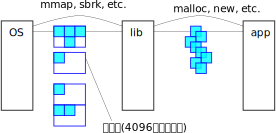
\includegraphics[width=0.7\textwidth]{out/pdf/svg/malloc_mmap.pdf}
  \end{center}
    
  \end{itemize}
\end{frame}

%%%%%%%%%%%%%%%%%

\section{ファイルシステム高速化のためのOSの機構}
%%%%%%%%%%%%%%%%%

%%%%%%%%%%%%%%%%% 
\subsection{キャッシュ}
%%%%%%%%%%%%%%%%%

%%%%%%%%%%%%%%%%% 
\begin{frame}
  \frametitle{キャッシュ}
  \begin{itemize}
  \item 一度読んだファイル(の一部分)をメモリ(キャッシュ)上に保持
  \item 一度書いたファイルもメモリ上に一定期間保持
  \item ファイル読み込み時,
    キャッシュ上にあるデータは2次記憶とのIOを行わずに返す
  \end{itemize}
\end{frame}

%%%%%%%%%%%%%%%%% 
\begin{frame}
  \frametitle{キャッシュが存在する理由}
  \begin{itemize}
  \item 2次記憶の性能 $\leq$ 主記憶の性能
  \item 性能の目安

    \begin{tabular}{|l|l|l|}\hline
             & 遅延     & 最大転送速度    \\\hline
      主記憶 & $10^{-7}$ & $10^{10}$〜$10^{11}$ bytes/sec \\
      SSD    & $10^{-5}$ & $10^{8}$〜$10^{9}$ bytes/sec \\
      HDD    & $10^{-2}$ & $10^{7}$〜$10^{8}$ bytes/sec \\\hline
    \end{tabular}
  \item 注: 最大転送速度は構成に大きく依存する
    \begin{itemize}
    \item HDDも多数並べる(RAID構成)ことで転送速度は稼げる
    \item 主記憶も同様で, 複数のモジュールを束ねて性能を出すのが普通
    \end{itemize}
  \end{itemize}
\end{frame}

%%%%%%%%%%%%%%%%% 
\begin{frame}
  \frametitle{キャッシュの動き}
  \begin{enumerate}
  \item <2-> read要求された部分がキャッシュ上にない$\rightarrow$
    \begin{enumerate}
    \item <3-> カーネル内にキャッシュのための領域を割り当て
    \item <4-> 2次記憶からキャッシュ上に読み込むとともに
    \item <5-> プロセス指定のメモリにもコピー
    \end{enumerate}
  \item <6-> read要求された部分がキャッシュ上にある$\rightarrow$
    \begin{enumerate}
    \item <7-> キャッシュからプロセス指定のメモリにコピー(高速)
    \end{enumerate}
  \end{enumerate}
  
  \begin{center}
    \only<1>{\includegraphics[width=0.6\textwidth]{out/pdf/svg/file_cache_1.pdf}}%
    \only<2>{\includegraphics[width=0.6\textwidth]{out/pdf/svg/file_cache_2.pdf}}%
    \only<3>{\includegraphics[width=0.6\textwidth]{out/pdf/svg/file_cache_3.pdf}}%
    \only<4>{\includegraphics[width=0.6\textwidth]{out/pdf/svg/file_cache_4.pdf}}%
    \only<5>{\includegraphics[width=0.6\textwidth]{out/pdf/svg/file_cache_5.pdf}}%
    \only<6>{\includegraphics[width=0.6\textwidth]{out/pdf/svg/file_cache_6.pdf}}%
    \only<7>{\includegraphics[width=0.6\textwidth]{out/pdf/svg/file_cache_7.pdf}}%
  \end{center}
\end{frame}

%%%%%%%%%%%%%%%%% 
\subsection{先読み}
%%%%%%%%%%%%%%%%%

%%%%%%%%%%%%%%%%% 
\begin{frame}
  \frametitle{先読みとは}
  \begin{itemize}
  \item プロセスが要求していない部分を先に(キャッシュ内に)読んでおくこと
  \item 実際問題としては, ファイルの読み出しが連続した部分に何回か行われた時点で発動
  \end{itemize}
\end{frame}

%%%%%%%%%%%%%%%%% 
\begin{frame}
  \frametitle{先読みの理由}
  \begin{itemize}
  \item<1-> 2次記憶の遅延が大
  \item<1-> 性能の目安再掲

    {\small\begin{tabular}{|l|l|l|}\hline
             & 遅延     & 最大転送速度    \\\hline
      主記憶 & $10^{-7}$ sec & $10^{10}$〜$10^{11}$ bytes/sec \\
      SSD    & $10^{-5}$ sec & $10^{8}$〜$10^{9}$ bytes/sec \\
      HDD    & $10^{-2}$ sec & $10^{7}$〜$10^{8}$ bytes/sec \\\hline
    \end{tabular}}
  \item<2-> \ao{小さなデータも「遅延」はほとんど同じ}
  \item<4-> e.g., $10^{-2}$ sec の遅延で 100MB/sec の転送速度は
    \[ 100 \mbox{MB/sec} \times 10^{-2} = 1 \mbox{MB/sec} \]
    以上の読み出しの場合のみ達成
  \end{itemize}

  \begin{center}
    \only<1-2>{\includegraphics[width=0.9\textwidth]{out/pdf/svg/prefetch_1.pdf}}%
    \only<3->{\includegraphics[width=0.9\textwidth]{out/pdf/svg/prefetch_3.pdf}}%
  \end{center}
\end{frame}

%%%%%%%%%%%%%%%%% 
\begin{frame}
  \frametitle{先読みの動作}
  \begin{itemize}
  \item 始めはプロセスが(readで)要求したサイズをそのまま2次記憶装置に要求
  \item 逐次的な読み出し(連続したオフセット)を検出すると,
    大きな読み出しを2次記憶装置に発行
  \end{itemize}
  \begin{center}
    \only<1>{\includegraphics[width=0.7\textwidth]{out/pdf/svg/prefetch_action_1.pdf}}%
    \only<2>{\includegraphics[width=0.7\textwidth]{out/pdf/svg/prefetch_action_2.pdf}}%
    \only<3>{\includegraphics[width=0.7\textwidth]{out/pdf/svg/prefetch_action_3.pdf}}%
    \only<4>{\includegraphics[width=0.7\textwidth]{out/pdf/svg/prefetch_action_4.pdf}}%
    \only<5>{\includegraphics[width=0.7\textwidth]{out/pdf/svg/prefetch_action_5.pdf}}%
    \only<6>{\includegraphics[width=0.7\textwidth]{out/pdf/svg/prefetch_action_6.pdf}}%
    \only<7>{\includegraphics[width=0.7\textwidth]{out/pdf/svg/prefetch_action_7.pdf}}%
    \only<8>{\includegraphics[width=0.7\textwidth]{out/pdf/svg/prefetch_action_8.pdf}}%
    \only<9>{\includegraphics[width=0.7\textwidth]{out/pdf/svg/prefetch_action_9.pdf}}%
    \only<10>{\includegraphics[width=0.7\textwidth]{out/pdf/svg/prefetch_action_10.pdf}}%
    \only<11>{\includegraphics[width=0.7\textwidth]{out/pdf/svg/prefetch_action_11.pdf}}%
  \end{center}
\end{frame}

%%%%%%%%%%%%%%%%%
\iffalse
\begin{frame}
  \frametitle{キャッシュ, 先読みの動作とアプリケーション性能への帰結}
  \begin{itemize}
  \item 以下のようなアプリケーションの性能について注意が必要
  \item 巨大: 扱うデータが巨大で主記憶に全て収まらない(または収めたくないほどには大きい)
  \item 索引: 全てのデータをアクセスせずに処理を
  \end{itemize}
\end{frame}
\fi

%%%%%%%%%%%%%%%%% 
\section{mmapの実装, 主記憶と2次記憶の統合}
%%%%%%%%%%%%%%%%%

%%%%%%%%%%%%%%%%%
\begin{frame}[fragile]
  \frametitle{復習: mmapの効果}
  \begin{itemize}
  \item 動作
\begin{lstlisting}
char * @{\it a}@ = mmap(0, @{\it sz}@, @{\it proto}@, @{\it flags}@, @{\it fd}@, @{\it offs}@);
\end{lstlisting}
で, アドレス範囲 $[a, a+\mbox{\it sz})$ が, ファイルの
範囲$[\mbox{\it offs}, \mbox{\it offs} + \mbox{\it sz})$に「対応(マップ)」される
\item つまり
  \begin{enumerate}
  \item {\tt $a$[$i$]}を読むとファイルの$(\mbox{\it offs} + i)$バイト目が読み出せる
  \item {\it flags} $=$ {\tt MAP\_SHARED|$\cdots$} ならば
    \begin{enumerate}
    \item {\tt a[$i$]}に書き込むと,
      ファイルの$(\mbox{\it offs} + i)$バイト目に書き込める
    \item 複数のプロセスが同じファイルの同じ場所をマップした場合,
      それらが書いた結果も共有される\ao{(プロセス間共有メモリ)}
    \end{enumerate}
  \end{enumerate}
  \end{itemize}
\end{frame}

%%%%%%%%%%%%%%%%%
\begin{frame}[fragile]
  \frametitle{mmapの実装 (\ldots はこうぢゃないよ)}
  \begin{itemize}
  \item 1. だけであれば, 以下と「意味的には」同じこと
    (説明の簡潔さのためreadがszバイト未満でリターンした場合の処理は省略)
\begin{lstlisting}
char * a = mmap(0, @{\it sz}@, @{\it proto}@, @{\it flags}@, @{\it fd}@, @{\it offs}@);
\end{lstlisting}
$\approx$
\begin{lstlisting}
char * a = malloc(sz);
read(fd, a, sz);
\end{lstlisting}
\item 2. ({\tt MAP\_SHARED}の動作)はそれでは済まない
\item 1. を含め, mmapはOSの仮想記憶管理の仕組みの拡張として以下のように
  (エレガントに)実装されている
\end{itemize}
\end{frame}

%%%%%%%%%%%%%%%%%
\begin{frame}[fragile]
  \frametitle{mmapの実装 概要}
  \begin{itemize}
  \item mmap呼び出し時
\begin{lstlisting}
char * a = mmap(0, @{\it sz}@, @{\it proto}@, @{\it flags}@, @{\it fd}@, @{\it offs}@);
\end{lstlisting}
\begin{enumerate}
\item $[\mbox{\tt a}, \mbox{\tt a} + \mbox{\it sz})$を論理的に割当てる
  (アドレス空間記述表に記述)
\item \ao{ファイルとの対応関係も記録しておく}
\item ページテーブル上では$[\mbox{\tt a}, \mbox{\tt a} + \mbox{\it sz})$に対応する
  ページは「不在」としておく(通常の要求時ページングと同じ)
\end{enumerate}
\item ページフォルト発生時
  \begin{itemize}
  \item アドレス空間記述表を見て, mmapでファイルに対応した領域であれば,
    ファイルの対応する領域を読み込む
  \end{itemize}
\end{itemize}
\end{frame}


%%%%%%%%%%%%%%%%% 
\begin{frame}
  \frametitle{復習: mmap以前のメモリ管理動作図}
  \begin{center}
    \only<1>{\includegraphics[width=1.0\textwidth]{out/pdf/svg/mem_management_1.pdf}}%
    \only<2>{\includegraphics[width=1.0\textwidth]{out/pdf/svg/mem_management_2.pdf}}%
    \only<3>{\includegraphics[width=1.0\textwidth]{out/pdf/svg/mem_management_3.pdf}}%
    \only<4>{\includegraphics[width=1.0\textwidth]{out/pdf/svg/mem_management_4.pdf}}%
    \only<5>{\includegraphics[width=1.0\textwidth]{out/pdf/svg/mem_management_5.pdf}}%
    \only<6>{\includegraphics[width=1.0\textwidth]{out/pdf/svg/mem_management_6.pdf}}%
%    \only<7>{\includegraphics[width=1.0\textwidth]{out/pdf/svg/mem_management_7.pdf}}%
%    \only<8>{\includegraphics[width=1.0\textwidth]{out/pdf/svg/mem_management_8.pdf}}%
  \end{center}
\end{frame}

%%%%%%%%%%%%%%%%% 
\begin{frame}
  \frametitle{mmap動作図}
  \begin{center}
    \only<1>{\includegraphics[width=1.0\textwidth]{out/pdf/svg/mmap_action_1.pdf}}%
    \only<2>{\includegraphics[width=1.0\textwidth]{out/pdf/svg/mmap_action_2.pdf}}%
    \only<3>{\includegraphics[width=1.0\textwidth]{out/pdf/svg/mmap_action_3.pdf}}%
    \only<4>{\includegraphics[width=1.0\textwidth]{out/pdf/svg/mmap_action_4.pdf}}%
    \only<5>{\includegraphics[width=1.0\textwidth]{out/pdf/svg/mmap_action_5.pdf}}%
    \only<6>{\includegraphics[width=1.0\textwidth]{out/pdf/svg/mmap_action_6.pdf}}%
    \only<7>{\includegraphics[width=1.0\textwidth]{out/pdf/svg/mmap_action_7.pdf}}%
  \end{center}
\end{frame}

%%%%%%%%%%%%%%%%% 
\begin{frame}
  \frametitle{要するに}
  \begin{itemize}
  \item mmapがなくてもOSは以下のことをやっていた
    \begin{itemize}
    \item プロセスに割り当てた領域でも, 実際に物理ページが対応しているとは限らない
    \item 物理ページが対応していないページへのアクセス $\rightarrow$ ページフォルト $\rightarrow$
      \begin{itemize}
      \item 物理メモリを割り当て
      \item 中身は, 初めてであれば0で埋める, そうでなければ
        \ao{2次記憶 (ページング領域, スワップ領域)}から読み込む
      \end{itemize}
    \end{itemize}
  \item \ao{mmapは, ページング領域として任意のファイルを指定できるようにした}に過ぎない
  \end{itemize}


\begin{center}
  \includegraphics[width=0.2\textwidth]{out/pdf/img/hirameki_woman.pdf}
  \includegraphics[width=0.2\textwidth]{out/pdf/img/kotowaza_mekara_uroko_man.pdf}
\end{center}  
\end{frame}


%%%%%%%%%%%%%%%%% 
\begin{frame}[fragile]
  \frametitle{OS内のページフォルト処理 (mmapなし)}
\begin{lstlisting}
handle_page_fault(void * a, access_type rw) {
  そのプロセスのアドレス空間記述表を見る;
  if (aへのアクセスrwは非合法) segmentation fault発生;
  p = 空いている物理ページ;


  if (aへのアクセスは初めて) {
    pを0で埋める;
  } else {
    aの中身を@\ao{ページング領域}@から読み込み, pをそれで埋める;
  }
  仮想アドレスa @$\rightarrow$@ pを対応(ページテーブル書き換え);
}
\end{lstlisting}
\begin{center}
  \includegraphics[width=0.2\textwidth]{out/pdf/img/hirameki_woman.pdf}
  \includegraphics[width=0.2\textwidth]{out/pdf/img/kotowaza_mekara_uroko_man.pdf}
\end{center}
\end{frame}

%%%%%%%%%%%%%%%%% 
\begin{frame}[fragile]
  \frametitle{OS内のページフォルト処理 (mmapあり)}
\begin{lstlisting}
handle_page_fault(void * a, access_type rw) {
  そのプロセスのアドレス空間記述表を見る;
  if (aへのアクセスrwは非合法) segmentation fault発生;
  p = 空いている物理ページ;
  if (@\ao{aはmmapでファイルと関連付けられた領域}@) {
    aの中身を@\ao{関連付けらたファイル}@から読み込み, pをそれで埋める;
  } else if (aへのアクセスは初めて) {
    pを0で埋める;
  } else {
    aの中身をページング領域から読み込み, pをそれで埋める;
  }
  仮想アドレスa @$\rightarrow$@ pを対応(ページテーブル書き換え);
}
\end{lstlisting}
\begin{center}
  \includegraphics[width=0.2\textwidth]{out/pdf/img/hirameki_woman.pdf}
  \includegraphics[width=0.2\textwidth]{out/pdf/img/kotowaza_mekara_uroko_man.pdf}
\end{center}  
\end{frame}

%%%%%%%%%%%%%%%%% 
\begin{frame}[fragile]
  \frametitle{共有マッピングとプライベートマッピング}
  \begin{itemize}
  \item 復習
    \begin{lstlisting}
char * a = mmap(0, @{\it sz}@, @{\it proto}@, @\ao{\it flags}@, @{\it fd}@, @{\it offs}@);
\end{lstlisting}

\item \ao{共有マッピング} (\ao{\it flags} $=$ {\tt MAP\_SHARED|...})
  \begin{itemize}
  \item 書き込みがファイルに反映される
  \item 複数プロセス間でも書き込みが共有される
  \end{itemize}
\item \ao{プライベートマッピング} (\ao{\it flags} $=$ {\tt MAP\_PRIVATE|...})
  \begin{itemize}
  \item 書き込みはファイルに反映されない
  \item 複数プロセス間でも書き込みは共有されない
  \end{itemize}
\item 違いは, \ao{物理メモリをどう使うか}の違いで, もたらされる
\end{itemize}
\end{frame}

%%%%%%%%%%%%%%%%%
\begin{frame}
  \frametitle{mmapの物理メモリ利用}
  \begin{itemize}
  \item {\tt MAP\_SHARED}
    \begin{itemize}
    \item 同じ場所(ファイル$+$オフセット)に対しては,
      同じ物理アドレス(物理ページ)を用いる
    \item 実はキャッシュと同じ物理ページ
    \end{itemize}
  \item<2-> {\tt MAP\_PRIVATE}
    \begin{itemize}
    \item (一般には) 同じ場所に対しても, 異なる物理アドレス(ページ)を用いる必要がある
    \item しかし, 「書き込みが実際に起きるまでは」同じ物理ページを用いる
      \ao{(コピーオンライト copy-on-write)}
    \end{itemize}
  \item<5-> 復習: read (各プロセスが異なる物理ページを用いる)
  \end{itemize}

  \begin{center}
  \only<1>{\includegraphics[width=0.6\textwidth]{out/pdf/svg/file_cache_8.pdf}}%
  \only<2>{\includegraphics[width=0.6\textwidth]{out/pdf/svg/file_cache_9.pdf}}%
  \only<3>{\includegraphics[width=0.6\textwidth]{out/pdf/svg/file_cache_10.pdf}}%
  \only<4>{\includegraphics[width=0.6\textwidth]{out/pdf/svg/file_cache_11.pdf}}%
  \only<5>{\includegraphics[width=0.6\textwidth]{out/pdf/svg/file_cache_12.pdf}}%
  \end{center}
\end{frame}

%%%%%%%%%%%%%%%%% 
\begin{frame}
  \frametitle{コピーオンライト}
  \begin{itemize}
  \item 「変更されるまでは物理メモリを共有する」方式の呼称
  \item<1-> 物理ページを共有しつつ, MMUの機能で「書き込み不可」属性をつけておく
  \item<2-> 書き込み時に保護例外が発生 $\rightarrow$ OSが対応する物理メモリをコピーし,
    「書き込まれたページ $\rightarrow$ 新しい物理ページ」にマッピングを変更
  \end{itemize}
  \begin{center}
    \only<1>{\includegraphics[width=0.8\textwidth]{out/pdf/svg/file_cache_9.pdf}}%
    \only<2>{\includegraphics[width=0.8\textwidth]{out/pdf/svg/file_cache_10.pdf}}%
    \only<3>{\includegraphics[width=0.8\textwidth]{out/pdf/svg/file_cache_11.pdf}}%
\end{center}
\end{frame}

%%%%%%%%%%%%%%%%% 
\begin{frame}
  \frametitle{mmapが効果的な場面(1)}
  \begin{itemize}
  \item 大きなファイルのごく一部を飛び飛びにアクセスする
    \begin{enumerate}
    \item lseek $+$ read (またはpread)で明示的に一部だけを
      アクセスするのは面倒
    \item といってファイルの全てをメモリに読み込むのは無駄
    \end{enumerate}
    $\Rightarrow$ mmapでファイル全体をマップする
    
  \item 典型例: 大きなデータの索引(index)
    \begin{itemize}
    \item 2分探索のための整列された配列
    \item 探索木(2分探索木, B木等)
    \item ハッシュ表
    \end{itemize}
  \end{itemize}
\end{frame}


%%%%%%%%%%%%%%%%% 
\begin{frame}
  \frametitle{mmapが効果的な場面(2)}
  \begin{itemize}
  \item 多く($P$個)のプロセスが同じファイルをアクセスする
    \begin{itemize}
    \item mmap (共有マッピング) $\rightarrow$ 同一領域に対する物理ページは共有
    \item mmap (プライベートマッピング)
      $\rightarrow$ 書き込まれていない領域に対する物理ページは共有
    \item read $\rightarrow$ 読み込んだプロセスごとに異なる物理ページ
    \end{itemize}
  \end{itemize}
\end{frame}

%%%%%%%%%%%%%%%%% 
\begin{frame}
  \frametitle{mmapが効果的な場面(3)}
  \begin{itemize}
  \item プログラム(命令)の読み込み
  \item 特に, 多くのプログラムが用いる大きなライブラリ (GUIなど)
  \item (1), (2)の性質を併せ持つ
  \end{itemize}
\end{frame}

%%%%%%%%%%%%%%%%% 
\begin{frame}
  \frametitle{{\tiny 直接ファイルシステムの話ではないが}プログラム起動の高速化}
  \begin{itemize}
  \item Unixにおけるプログラム起動 $\approx$
    \begin{enumerate}
    \item fork (アドレス空間の複製)
    \item execv (プログラムの実行)
      \begin{enumerate}
      \item 指定された実行可能ファイルを読み込み
      \item 共有ライブラリを読み込み
      \end{enumerate}
    \end{enumerate}
  \item 高速化
    \begin{itemize}
    \item fork時に, 物理メモリを親プロセス, 子プロセスで共有\ao{(コピーオンライト)}
      \begin{itemize}
      \item すぐにexecvされれば, 子プロセスのマッピングは解除
      \end{itemize}
    \item 共有ライブラリを\ao{mmapで読み込み}
    \end{itemize}
  \end{itemize}
\end{frame}


\end{document}


%%%%%%%%%%%%%%%%% 
\begin{frame}[fragile]
  \frametitle{read vs. mmap}
  

\end{frame}

%%%%%%%%%%%%%%%%% 
\begin{frame}
  \frametitle{mmap API}
  \begin{itemize}
  \item {\tt void * {\it a} = mremap({\it addr}, {\it len}, {\it new\_len}, {\it flags}{\rm [, {\it new\_addr}]});}
  \item {\tt void * {\it a} = munmap({\it addr}, {\it len});}
  \end{itemize}
\end{frame}

%%%%%%%%%%%%%%%%% 
\begin{frame}
  \frametitle{ファイル名, パス名}
  \begin{itemize}
  \item 
  \end{itemize}
\end{frame}

%%%%%%%%%%%%%%%%% 
\begin{frame}
  \frametitle{標準入出力}
\end{frame}

%%%%%%%%%%%%%%%%% 
\begin{frame}
  \frametitle{ファイルディスクリプタの複製}
\end{frame}


\end{document}
